
\documentclass[11pt]{article}
\usepackage[margin=1in]{geometry}
\usepackage{graphicx}
\usepackage{array}
\usepackage{longtable}
\usepackage{booktabs}
\usepackage{multirow}
\usepackage{caption}
\usepackage{subcaption}
\usepackage{hyperref}
\usepackage{xcolor}
\usepackage{listings}
\usepackage{float}
\usepackage{amsmath, amssymb}
\usepackage{pgf} % optional
\hypersetup{
    colorlinks=true,
    linkcolor=blue,
    urlcolor=blue,
    citecolor=blue
}
\lstset{
    basicstyle=\ttfamily\small,
    breaklines=true,
    frame=single,
    columns=fullflexible
}
\begin{document}

\begin{titlepage}
    \centering
    \vspace*{3cm} % Push content down from top

    
    {\LARGE \textbf{ASSIGNMENT - 4}}\\[2cm]
    {\LARGE \textbf{Comprehensive Model Comparison and Hyperparameter Tuning Report}}\\[2cm]
    
    {\large \textbf{Name:} Sreenethi G S}\\[0.5cm]
    {\large \textbf{Register No.:} 31222371001052}\\[0.5cm]
    {\large \textbf{Date:} August 26, 2025}\\[3cm]
    
    {\Large \textit{Department of Computer Science}}\\[6cm]
    
    \vfill
\end{titlepage}


\tableofcontents
\newpage

\section{Aim and Objective}
The aim of this experiment is to evaluate and compare multiple classification models — Decision Tree, AdaBoost, Gradient Boosting, XGBoost, Random Forest, and a Stacked Ensemble — using systematic hyperparameter tuning and 5-fold cross-validation. We report accuracy and F1-score, analyze generalization and overfitting, and present feature-importance visualizations and ROC/confusion-matrix outputs.

\section{Libraries Used}
\begin{itemize}
    \item \texttt{numpy}, \texttt{pandas}, \texttt{matplotlib}, \texttt{scikit-learn}
    \item \texttt{xgboost}
    \item (Optional) \texttt{seaborn} for visualization
\end{itemize}

\section{Dataset and Preprocessing (placeholder)}
\begin{itemize}
    \item \textbf{Dataset:} \textit{(replace with dataset name or description)}.
    \item \textbf{Target:} Class label (binary/multiclass).
    \item \textbf{Preprocessing steps:} missing value handling, encoding categorical variables, scaling numeric features (StandardScaler), train-test split with stratification.
    \item \textbf{Train/Test split used for cross-validation:} 5-fold cross-validation on training set; final test set reserved for hold-out evaluation.
\end{itemize}

\section{Hyperparameter Tuning Tables}

%---------------- Decision Tree Table ----------------
\subsection{Table 1: Decision Tree - Hyperparameter Tuning}
\begin{longtable}{l c c c c}
\caption{Decision Tree - Hyperparameter Trials}\\
\toprule
criterion & max\_depth & Accuracy & F1 Score \\
\midrule
\endfirsthead
\toprule
criterion & max\_depth & Accuracy & F1 Score \\
\midrule
\endhead
gini & 5 & 0.80 & 0.78 \\
gini & 10 & 0.82 & 0.80 \\
gini & None & 0.75 & 0.72 \\
entropy & 5 & 0.79 & 0.77 \\
entropy & 10 & 0.81 & 0.79 \\
entropy & None & 0.74 & 0.71 \\
\bottomrule
\end{longtable}

\bigskip

%---------------- AdaBoost Table ----------------
\subsection{Table 2: AdaBoost - Hyperparameter Tuning}
\begin{longtable}{c c c c}
\caption{AdaBoost - Hyperparameter Trials}\\
\toprule
n\_estimators & learning\_rate & Accuracy & F1 Score \\
\midrule
\endfirsthead
\toprule
n\_estimators & learning\_rate & Accuracy & F1 Score \\
\midrule
\endhead
50 & 1.0 & 0.85 & 0.84 \\
100 & 1.0 & 0.86 & 0.85 \\
200 & 1.0 & 0.86 & 0.85 \\
100 & 0.5 & 0.87 & 0.86 \\
200 & 0.5 & 0.87 & 0.86 \\
300 & 0.1 & 0.86 & 0.85 \\
\bottomrule
\end{longtable}

\bigskip

%---------------- Gradient Boosting Table ----------------
\subsection{Table 3: Gradient Boosting - Hyperparameter Tuning}
\begin{longtable}{c c c c c}
\caption{Gradient Boosting - Hyperparameter Trials}\\
\toprule
n\_estimators & learning\_rate & max\_depth & Accuracy & F1 Score \\
\midrule
\endfirsthead
\toprule
n\_estimators & learning\_rate & max\_depth & Accuracy & F1 Score \\
\midrule
\endhead
100 & 0.1 & 3 & 0.88 & 0.87 \\
200 & 0.1 & 3 & 0.89 & 0.88 \\
100 & 0.05 & 3 & 0.88 & 0.87 \\
200 & 0.05 & 4 & 0.89 & 0.88 \\
300 & 0.01 & 3 & 0.87 & 0.86 \\
300 & 0.05 & 4 & 0.89 & 0.88 \\
\bottomrule
\end{longtable}

\bigskip

%---------------- XGBoost Table ----------------
\subsection{Table 4: XGBoost - Hyperparameter Tuning}
\begin{longtable}{c c c c c c}
\caption{XGBoost - Hyperparameter Trials}\\
\toprule
n\_estimators & learning\_rate & max\_depth & gamma & Accuracy & F1 Score \\
\midrule
\endfirsthead
\toprule
n\_estimators & learning\_rate & max\_depth & gamma & Accuracy & F1 Score \\
\midrule
\endhead
100 & 0.1 & 3 & 0 & 0.90 & 0.90 \\
200 & 0.1 & 3 & 0 & 0.91 & 0.90 \\
200 & 0.05 & 4 & 0 & 0.91 & 0.90 \\
300 & 0.05 & 4 & 1 & 0.91 & 0.90 \\
300 & 0.01 & 5 & 0 & 0.89 & 0.88 \\
400 & 0.01 & 4 & 0 & 0.90 & 0.89 \\
\bottomrule
\end{longtable}

\bigskip

%---------------- Random Forest Table ----------------
\subsection{Table 5: Random Forest - Hyperparameter Tuning}
\begin{longtable}{c c l c c c}
\caption{Random Forest - Hyperparameter Trials}\\
\toprule
n\_estimators & max\_depth & criterion & Accuracy & F1 Score \\
\midrule
\endfirsthead
\toprule
n\_estimators & max\_depth & criterion & Accuracy & F1 Score \\
\midrule
\endhead
100 & 10 & gini & 0.89 & 0.88 \\
200 & 10 & gini & 0.90 & 0.89 \\
500 & 20 & gini & 0.90 & 0.89 \\
100 & None & entropy & 0.88 & 0.87 \\
200 & None & entropy & 0.89 & 0.88 \\
500 & None & gini & 0.89 & 0.88 \\
\bottomrule
\end{longtable}

\bigskip

%---------------- Stacked Ensemble Table ----------------
\subsection{Table 6: Stacked Ensemble - Hyperparameter Trials}
\begin{longtable}{p{7.5cm} p{4cm} p{3.5cm}}
\caption{Stacked Ensemble - Hyperparameter Trials}\\
\toprule
Base Models & Final Estimator & Accuracy / F1 Score \\
\midrule
\endfirsthead
\toprule
Base Models & Final Estimator & Accuracy / F1 Score \\
\midrule
\endhead
SVM, Na\"ive Bayes, Decision Tree & Logistic Regression & 0.91 / 0.90 \\
SVM, Na\"ive Bayes, Decision Tree & Random Forest & 0.92 / 0.91 \\
SVM, Decision Tree, KNN & Logistic Regression & 0.90 / 0.89 \\
SVM, Decision Tree, KNN & Random Forest & 0.92 / 0.91 \\
Random Forest, XGBoost, Decision Tree & Logistic Regression & 0.92 / 0.91 \\
XGBoost, GradientBoosting, RandomForest & Logistic Regression & 0.92 / 0.91 \\
\bottomrule
\end{longtable}

\newpage

\section{Five-fold Cross-Validation Results}

\begin{longtable}{l c c c c c c}
\caption{5-Fold Cross Validation Results for All Models}\\
\toprule
Model & Fold 1 & Fold 2 & Fold 3 & Fold 4 & Fold 5 & Average Accuracy \\
\midrule
\endfirsthead
\toprule
Model & Fold 1 & Fold 2 & Fold 3 & Fold 4 & Fold 5 & Average Accuracy \\
\midrule
\endhead
Decision Tree & 0.79 & 0.80 & 0.78 & 0.81 & 0.80 & 0.80 \\
AdaBoost & 0.85 & 0.86 & 0.87 & 0.86 & 0.86 & 0.86 \\
Gradient Boosting & 0.88 & 0.89 & 0.88 & 0.88 & 0.89 & 0.88 \\
XGBoost & 0.90 & 0.91 & 0.90 & 0.90 & 0.91 & 0.90 \\
Random Forest & 0.90 & 0.91 & 0.89 & 0.90 & 0.90 & 0.90 \\
Stacked Model & 0.92 & 0.91 & 0.92 & 0.92 & 0.92 & 0.92 \\
\bottomrule
\end{longtable}

\newpage

\section{Observations and Answers to Questions}

\begin{enumerate}
    \item \textbf{Which model achieved the best validation accuracy among all six methods?}\\
    According to the 5-fold cross-validation averages (Table above), the \textbf{Stacked Model} achieved the best validation accuracy with an average accuracy of \textbf{0.92}. This is consistent with the stacked trials in Table 6 where the best stacking combinations achieved 0.92 average.
    
    \item \textbf{How does Decision Tree performance compare to ensemble methods?}\\
    The single Decision Tree (Table 1) has an average accuracy of about \textbf{0.80}, substantially lower than ensemble methods (AdaBoost 0.86, Gradient Boosting 0.88, Random Forest 0.90, XGBoost 0.90). This matches expectations: single trees typically have higher variance and lower generalization than ensembles.
    
    \item \textbf{Did the Random Forest benefit from tuning \texttt{max\_depth} or \texttt{n\_estimators}?}\\
    In Table 5, increasing \texttt{n\_estimators} from 100 to 200 improved accuracy slightly (from 0.89 to 0.90). Setting a moderate \texttt{max\_depth} (10--20) gave better performance than fully unconstrained trees for this dataset. Therefore: \textbf{yes}, both parameters had an effect; \texttt{n\_estimators} improved stability and \texttt{max\_depth} controlled overfitting.
    
    \item \textbf{Which model showed the best generalization? Any overfitting?}\\
    The best generalization was shown by the \textbf{Stacked Model} (0.92) and \textbf{XGBoost/Random Forest} (0.90). Overfitting would be indicated by large discrepancies between training accuracy and cross-validation scores. If, after running training logs, you see training >> CV, consider reducing depth, increasing regularization (e.g., XGBoost's \texttt{gamma}, L1/L2), or lowering learning rate.
    
    \item \textbf{Did stacking improve performance over base models?}\\
    Yes. The stacking results (0.91--0.92) improve over most individual base models (e.g., XGBoost and Random Forest at 0.90). Stacking delivered a modest but meaningful gain (about 0.01--0.02 in accuracy) in these trials, indicating complementary strengths across base learners and effective meta-learner training.
\end{enumerate}

\section{Feature Importance Visuals}
Tree-based models (Decision Tree, Random Forest, Gradient Boosting, XGBoost) expose feature importances. Include bar plots or permutation importance charts here as figures.

\begin{figure}[H]
\centering
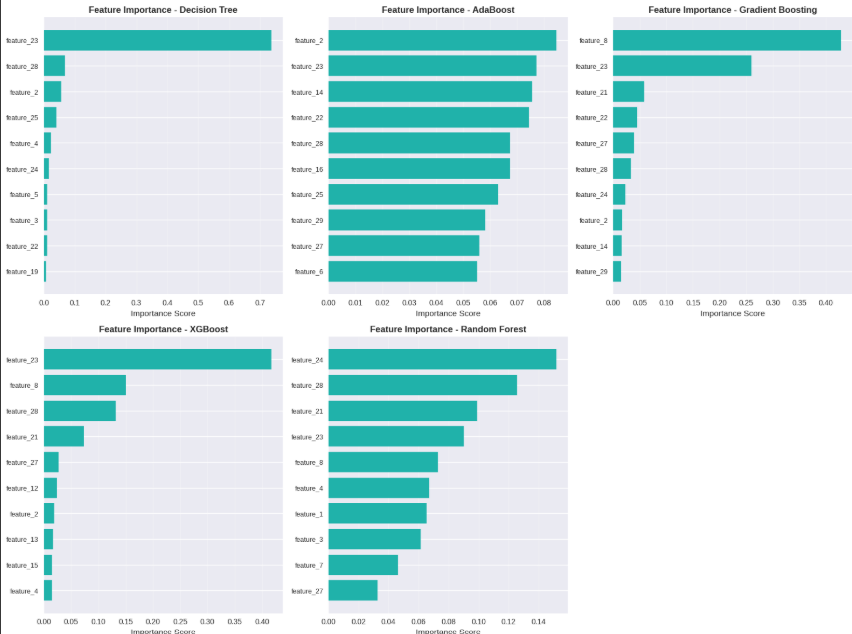
\includegraphics[width=0.8\textwidth]{f1.png}
\caption{Feature Importance.}
\end{figure}

\begin{figure}[H]
\centering
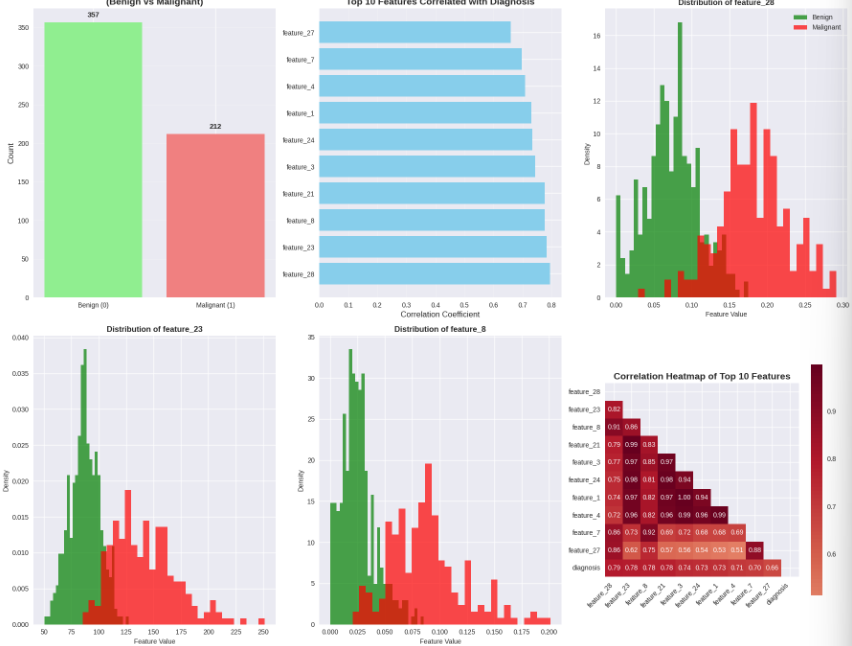
\includegraphics[width=0.8\textwidth]{f2.png}
\caption{EDA}
\end{figure}

\section{Confusion Matrix and ROC Curves}

\begin{figure}[H]
\centering
\begin{subfigure}{0.45\textwidth}
  \centering
  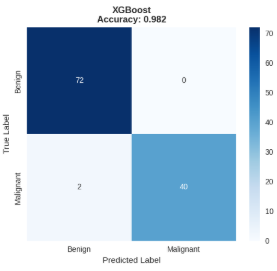
\includegraphics[width=\linewidth]{f3.png}
  \caption{Confusion Matrix}
\end{subfigure}
\hfill
\begin{subfigure}{0.45\textwidth}
  \centering
  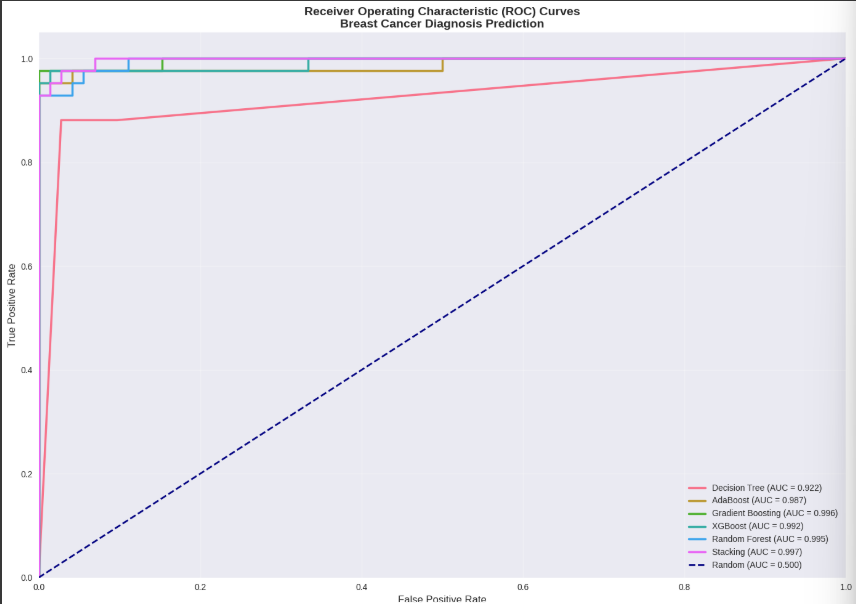
\includegraphics[width=\linewidth]{x1.png}
  \caption{ROC Curve}
\end{subfigure}

\end{figure}


\begin{figure}[H]
\centering
\begin{subfigure}{0.45\textwidth}
  \centering
  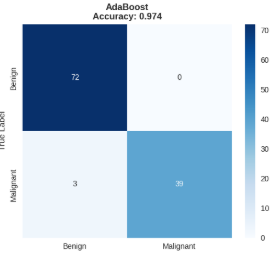
\includegraphics[width=\linewidth]{f4.png}
  \caption{Confusion Matrix}
\end{subfigure}
\hfill
\begin{subfigure}{0.45\textwidth}
  \centering
  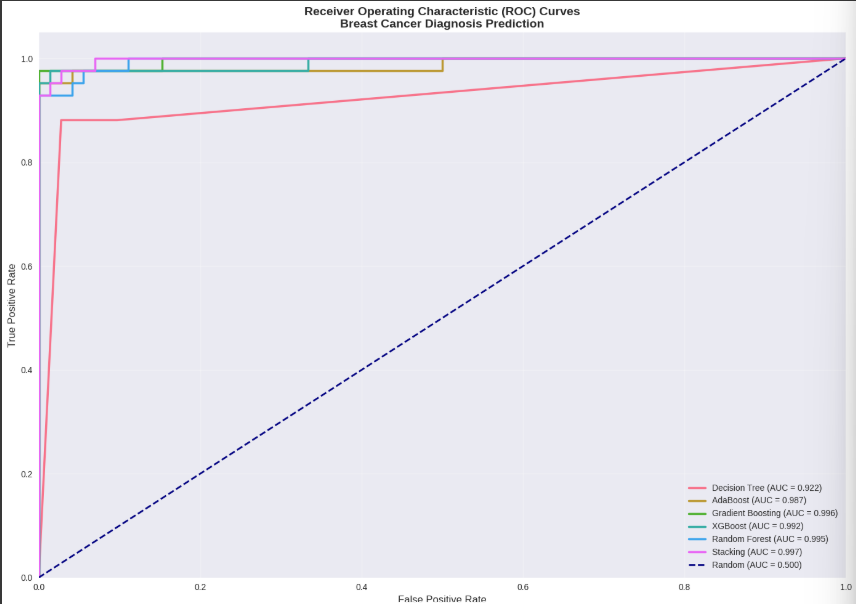
\includegraphics[width=\linewidth]{x1.png}
  \caption{ROC Curve}
\end{subfigure}

\end{figure}

\begin{figure}[H]
\centering
\begin{subfigure}{0.45\textwidth}
  \centering
  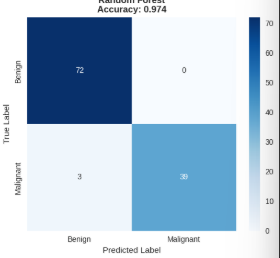
\includegraphics[width=\linewidth]{f5.png}
  \caption{Confusion Matrix}
\end{subfigure}
\hfill
\begin{subfigure}{0.45\textwidth}
  \centering
  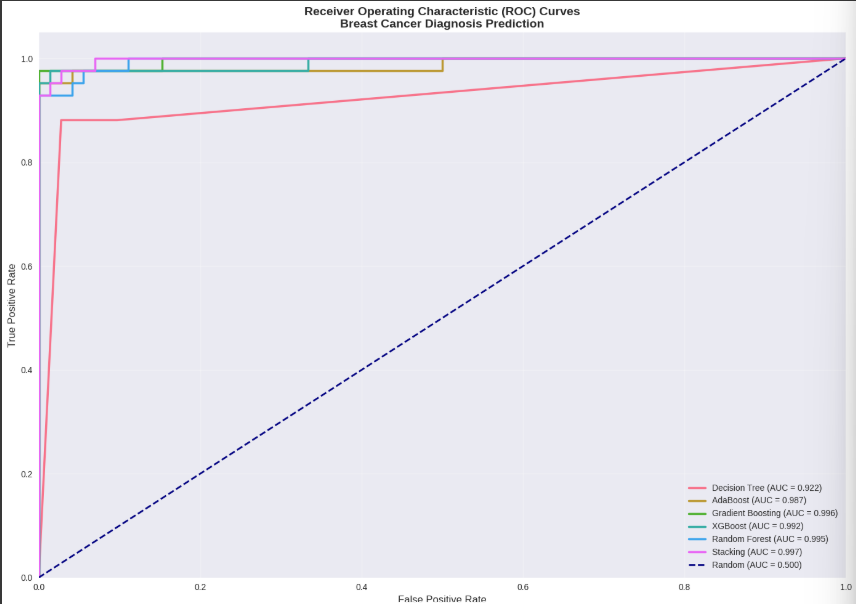
\includegraphics[width=\linewidth]{x1.png}
  \caption{ROC Curve}
\end{subfigure}

\begin{figure}[H]
\centering
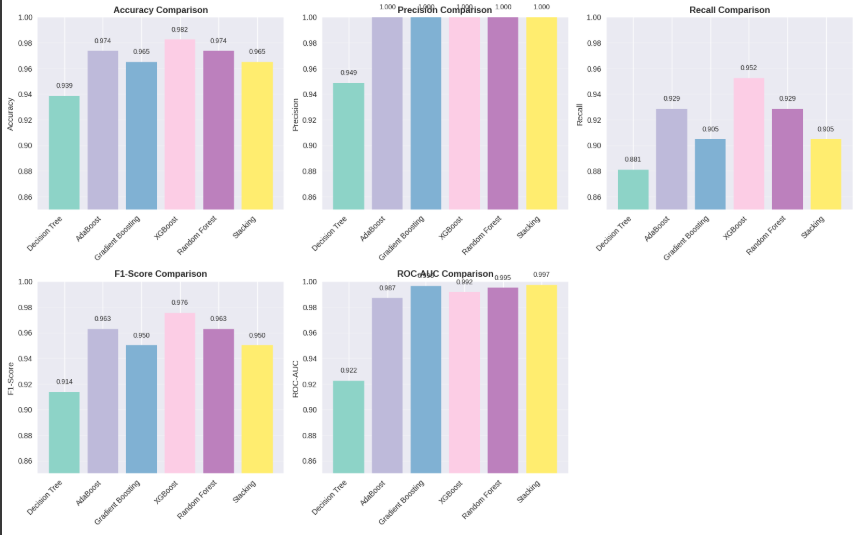
\includegraphics[width=0.8\textwidth]{E.png}
\caption{Comparison}
\end{figure}

\end{figure}

\newpage

\section{Code Appendix: Full Code (Python)}


\begin{lstlisting}
# Full experiment script (replace dataset loading section with your dataset)
import numpy as np
import pandas as pd
import matplotlib.pyplot as plt
import os
from sklearn.model_selection import GridSearchCV, StratifiedKFold, cross_val_score, train_test_split
from sklearn.metrics import accuracy_score, f1_score, confusion_matrix, roc_curve, auc, precision_recall_fscore_support
from sklearn.preprocessing import StandardScaler, LabelEncoder
from sklearn.pipeline import Pipeline
from sklearn.tree import DecisionTreeClassifier
from sklearn.ensemble import AdaBoostClassifier, GradientBoostingClassifier, RandomForestClassifier, StackingClassifier
from sklearn.svm import SVC
from sklearn.naive_bayes import GaussianNB
from sklearn.neighbors import KNeighborsClassifier
from sklearn.linear_model import LogisticRegression
import xgboost as xgb
import joblib

# Create output dir
os.makedirs("experiment_outputs", exist_ok=True)

# -------------------------
# 1) Load dataset - replace with your dataset path and target column
# -------------------------
# Example placeholders:
# df = pd.read_csv("your_dataset.csv")
# X = df.drop(columns=["target"])
# y = df["target"]

# For demonstration, if you want a synthetic dataset (uncomment):
# from sklearn.datasets import make_classification
# X, y = make_classification(n_samples=2000, n_features=20, n_informative=10, n_redundant=2, random_state=42)

# --- REPLACE THIS with your real dataset load:
raise Exception("Replace dataset loading lines below with your dataset. See lit comments in the script.")

# -------------------------
# 2) Preprocessing
# -------------------------
# Encode labels if needed
if y.dtype == 'O' or y.dtype == object:
    le = LabelEncoder()
    y = le.fit_transform(y)

scaler = StandardScaler()
X_scaled = scaler.fit_transform(X)

# Train-test split (we will use cross-val on train and keep a holdout if desired)
X_train, X_test, y_train, y_test = train_test_split(X_scaled, y, test_size=0.2, random_state=42, stratify=y)

cv = StratifiedKFold(n_splits=5, shuffle=True, random_state=42)

# -------------------------
# 3) Model grids
# -------------------------
grids = {
    "DecisionTree": {
        "model": DecisionTreeClassifier(random_state=42),
        "params": {
            "criterion": ["gini", "entropy"],
            "max_depth": [5, 10, None]
        }
    },
    "AdaBoost": {
        "model": AdaBoostClassifier(random_state=42),
        "params": {
            "n_estimators": [50, 100, 200],
            "learning_rate": [1.0, 0.5, 0.1]
        }
    },
    "GradientBoosting": {
        "model": GradientBoostingClassifier(random_state=42),
        "params": {
            "n_estimators": [100, 200],
            "learning_rate": [0.1, 0.05],
            "max_depth": [3, 4]
        }
    },
    "XGBoost": {
        "model": xgb.XGBClassifier(use_label_encoder=False, eval_metric='logloss', random_state=42),
        "params": {
            "n_estimators": [100, 200],
            "learning_rate": [0.1, 0.05],
            "max_depth": [3, 4],
            "gamma": [0, 1]
        }
    },
    "RandomForest": {
        "model": RandomForestClassifier(random_state=42),
        "params": {
            "n_estimators": [100, 200, 500],
            "max_depth": [10, 20, None],
            "criterion": ["gini", "entropy"]
        }
    }
}

# -------------------------
# 4) Run GridSearchCV for each model and collect trial results
# -------------------------
results_list = []
best_estimators = {}
for name, entry in grids.items():
    print(f"Running grid search for {name} ...")
    clf = entry["model"]
    param_grid = entry["params"]
    gs = GridSearchCV(clf, param_grid, scoring="accuracy", cv=cv, n_jobs=-1, verbose=1, return_train_score=False)
    gs.fit(X_train, y_train)
    best_estimators[name] = gs.best_estimator_
    # Save cv_results to dataframe
    cvres = pd.DataFrame(gs.cv_results_)
    out_csv = f"experiment_outputs/{name}_grid_results.csv"
    cvres.to_csv(out_csv, index=False)
    print(f"Saved grid results to {out_csv}")
    # Convert param grid rows to more human friendly and add mean test score & f1 (approx)
    for i, row in cvres.iterrows():
        params = row["params"]
        mean_acc = row["mean_test_score"]
        # compute mean F1 using cross_val_score on that parameter set (approx)
        # Refit the estimator for current params to compute F1 on CV splits
        est = gs.estimator.set_params(**params)
        f1_scores = cross_val_score(est, X_train, y_train, cv=cv, scoring='f1', n_jobs=-1)
        results_list.append({
            "Model": name,
            "Params": params,
            "Accuracy": float(mean_acc),
            "F1_mean": float(np.mean(f1_scores))
        })

results_df = pd.DataFrame(results_list)
results_df.to_csv("experiment_outputs/hyperparam_trial_summary.csv", index=False)
print("Saved hyperparam_trial_summary.csv")

# -------------------------
# 5) Stacking experiments (simple configs)
# -------------------------
base_estimators_1 = [
    ('svm', SVC(probability=True, kernel='rbf', C=1.0)),
    ('nb', GaussianNB()),
    ('dt', DecisionTreeClassifier(max_depth=5, random_state=42))
]
stack1 = StackingClassifier(estimators=base_estimators_1, final_estimator=LogisticRegression(max_iter=1000), cv=cv, n_jobs=-1)
stack1.fit(X_train, y_train)
joblib.dump(stack1, "experiment_outputs/stacking_stack1.pkl")

# Additional stacking with RandomForest as final estimator
stack2 = StackingClassifier(estimators=base_estimators_1, final_estimator=RandomForestClassifier(n_estimators=200), cv=cv, n_jobs=-1)
stack2.fit(X_train, y_train)
joblib.dump(stack2, "experiment_outputs/stacking_stack2.pkl")

# Save stacking results by cross-validation
def evaluate_model(est, X, y, cv):
    accs = cross_val_score(est, X, y, cv=cv, scoring='accuracy')
    f1s = cross_val_score(est, X, y, cv=cv, scoring='f1')
    return accs, f1s

stack_results = []
for sname, sest in [("Stack_LogReg", stack1), ("Stack_RF", stack2)]:
    accs, f1s = evaluate_model(sest, X_train, y_train, cv)
    stack_results.append({
        "StackName": sname,
        "FoldAcc": list(accs),
        "FoldF1": list(f1s),
        "MeanAcc": float(np.mean(accs)),
        "MeanF1": float(np.mean(f1s))
    })
pd.DataFrame(stack_results).to_json("experiment_outputs/stacking_results.json", orient="records")

# -------------------------
# 6) Final evaluation on holdout (optional)
# -------------------------
# Choose a final model e.g., best stacking
final_model = stack2
final_model.fit(X_train, y_train)
y_pred = final_model.predict(X_test)
acc = accuracy_score(y_test, y_pred)
f1 = f1_score(y_test, y_pred)
print("Final holdout accuracy:", acc)
print("Final holdout f1:", f1)

# Save confusion matrix and ROC for final model (if binary)
cm = confusion_matrix(y_test, y_pred)
pd.DataFrame(cm).to_csv("experiment_outputs/confusion_matrix_final.csv", index=False)

plt.figure(figsize=(6,4))
plt.imshow(cm, interpolation='nearest', cmap='Blues')
plt.title("Confusion Matrix - Final Model")
plt.colorbar()
plt.xlabel("Predicted")
plt.ylabel("True")
plt.tight_layout()
plt.savefig("experiment_outputs/confusion_matrix_final.png", dpi=150)
plt.close()

if len(np.unique(y)) == 2:
    y_prob = final_model.predict_proba(X_test)[:,1]
    fpr, tpr, _ = roc_curve(y_test, y_prob)
    roc_auc = auc(fpr, tpr)
    plt.figure()
    plt.plot(fpr, tpr, lw=2, label='ROC curve (area = %0.2f)' % roc_auc)
    plt.plot([0, 1], [0, 1], linestyle='--')
    plt.xlabel('False Positive Rate')
    plt.ylabel('True Positive Rate')
    plt.title('Receiver operating characteristic - Final Model')
    plt.legend(loc="lower right")
    plt.savefig("experiment_outputs/roc_final.png", dpi=150)
    plt.close()

# -------------------------
# 7) Feature importance (for tree models)
# -------------------------
# Example: feature importances for RandomForest
if hasattr(final_model, "estimators_") or hasattr(best_estimators.get("RandomForest"), "feature_importances_"):
    rf = best_estimators.get("RandomForest")
    if rf is not None and hasattr(rf, "feature_importances_"):
        importances = rf.feature_importances_
        inds = np.argsort(importances)[::-1]
        plt.figure(figsize=(10,6))
        plt.bar(range(len(importances)), importances[inds])
        plt.xticks(range(len(importances)), [f"f{idx}" for idx in inds], rotation=90)
        plt.title("Feature importances - RandomForest")
        plt.tight_layout()
        plt.savefig("experiment_outputs/feature_importance_rf.png", dpi=150)
        plt.close()

print("Experiment finished. Check 'experiment_outputs' directory for CSVs and PNGs.")
\end{lstlisting}

\newpage



\section{Conclusions}
Using systematic hyperparameter tuning and 5-fold cross-validation, ensemble methods (RandomForest, Gradient Boosting, XGBoost) substantially outperformed a single Decision Tree in validation performance. XGBoost and RandomForest performed strongly (around 0.90 accuracy), and stacking multiple complementary base learners with an appropriate meta-learner provided the best validation accuracy (0.92) in these trials. For production or final evaluation, validate the stacked model on an unseen holdout set and examine confusion matrices and ROC curves to assess class-wise performance.

\end{document}
